In this chapter, we examine the effect of including tetraquark operators on the spectrum in the scalar meson sectors containing the $K_0^*(700)$ (here and often elsewhere referred to as the $\kappa$) and the $a_0(980)$ in $N_f = 2 + 1$ QCD, using an anisotropic lattice with gauge field configurations generated by the Hadron Spectrum Collaboration~\cite{}. Preliminary results of  additional states found using tetraquark operators are shown, and possible implications of these states are discussed. This is the first work to study the tetraquarks in the $\kappa$ and $a_0(980)$ sectors of $N_f = 2 + 1$, $m_\pi \approx 230$ MeV QCD with proper evaluation of all diagrams in the correlator Wick contractions. Previous studies of the $\kappa$  have invalidly neglected the evaluation of disconnected contributions, and only one $N_f = 2 + 1$ study of the $a_0(980)$ to date, by Alexandrou et al.~\cite{}, has included disconnected diagrams. That study, done at $m_\pi \approx 300$ MeV, identified an additional tetraquark-associated level in the range of 1100 to 1200 MeV, which they claim to be a candidate for the $a_0(980)$ meson. We find an additional state in the range of ... to ...

\section{Operator construction}
We include single- and two- meson operators, as well as tetraquark operators, in the basis of interpolating operators. We construct our elemental operators using building blocks of smeared, gauge-covariantly displaced quark fields, and stout-smeared link variables. To form the final operators out of our elemental operators, we project the elemental operators onto various symmetry channels according to isospin, parity, $G$-parity, octahedral little group, etc. For example, to form a meson operator $M_{l}(t)$ that transforms irreducibly under all symmetries of interest (labeled by the compound index $l$) at time $t$, we must 
take a linear combination of our elemental meson operators, $M_{l}(t)=c_{\alpha \beta}^{(l)} \Phi_{\alpha \beta}^{A B}(\boldsymbol{p}, t)$. To form a two-meson operator $\mathcal{O}_l(t)$, we would follow a similar procedure and project the product of two final meson operators $M^{a}_{l_a}(t) M^{b}_{l_a}(t)$ onto a final symmetry channel $l$: $\mathcal{O}_l(t) = c^{(l)}_{l_a l_b} M^{a}_{l_a}(t) M^{b}_{l_a}(t)$. 

In order to construct a tetraquark operator, we must consider the various ways to construct a color-singlet four-quark object out of four quark fields. We can see from the Clebsch-Gordon decompositions that the only way to construct a color-singlet is with two quarks and two antiquarks, and that doing so yields two linearly independent color singlet objects:
\begin{equation}
\begin{array}{l}
    {3 \otimes 3 \otimes 3 \otimes 3=3\oplus3\oplus3\oplus\overline{6}\oplus\overline{6}\oplus15\oplus15\oplus15\oplus15},\\
    {3 \otimes 3 \otimes 3 \otimes \overline{3}=\overline{3}\oplus\overline{3}\oplus\overline{3}\oplus6\oplus6\oplus6\oplus\overline{15}\oplus\overline{15}\oplus24},\\
    {3 \otimes 3 \otimes \overline{3} \otimes \overline{3}=1\oplus1\oplus8\oplus8\oplus8\oplus8\oplus10\oplus\overline{10}\oplus27}.
\end{array}
\end{equation}
There are 81 basis vectors formed by the quark fields, $p_{\alpha}^{*}(x) q_{\beta}^{*}(x) r_{\gamma}(x) s_{\mu}(x)$, where each $r$, $s$ transforms as a color vector in the fundamental $3$ irrep, and so, $p^{*}$, $q^{*}$ transform in the $\overline 3$ irrep. We need two linearly independent and gauge-invariant combinations of these to exhaust all possible tetraquark operators. It is easy to see that the following combinations are both linearly independent and gauge-invariant (and thus form our elemental tetraquark operators):
\begin{equation}\label{eq:tsta}
\begin{aligned} T_{S} &=\left(\delta_{\alpha \gamma} \delta_{\beta \mu}+\delta_{\alpha \mu} \delta_{\beta \gamma}\right) p_{\alpha}^{*}(x) q_{\beta}^{*}(x) r_{\gamma}(x) s_{\mu}(x) \\ T_{A} &=\left(\delta_{\alpha \gamma} \delta_{\beta \mu}-\delta_{\alpha \mu} \delta_{\beta \gamma}\right) p_{\alpha}^{*}(x) q_{\beta}^{*}(x) r_{\gamma}(x) s_{\mu}(x).\end{aligned}
\end{equation}
While these elemental tetraquark operators each ostensibly appear to be a combination of two individual mesons, they differ in that the gauge-invariant pieces do need to transform irreducibly under symmetry operations; only the combination of the two quark-antiquark pairs must transform irreducibly. In other words, we project the entire elemental tetraquark operator onto relevant symmetry channels, rather than each individual ``meson'' operator.
\section{Lattice Spectra Results (Preliminary)}
\subsection{$\kappa$ Channel}
We summarize results obtained by fitting a spectrum in the $\kappa$ at-rest symmetry channel for two operator bases: one including only single-meson and two-meson operators, and one including single-meson, two-meson, and tetraquark operators. Figure \ref{fig:kappa_spectrum} shows the spectrum with and without the inclusion of a tetraquark operator in the basis. The tetraquark operator is of the flavor structure \textit{antistrange-light-antistrange-strange}, and was of the antisymmetric form in (\ref{eq:tsta}). We see that including a tetraquark operator yields an additional state not present when only single- and two-meson operators are used. Additionally, a plot of the overlap factors for the tetraquark operator (Figure~\ref{fig:zkappa}) shows significant overlap onto this extra state. This suggests that there is a state in our lattice spectrum that shares quantum numbers with the $\kappa$ resonance, and that has tetraquark content. Whether or not this is evidence of the $\kappa$ resonance having tetraquark content, however, will have to wait for future scattering studies using this data.
\begin{figure}
  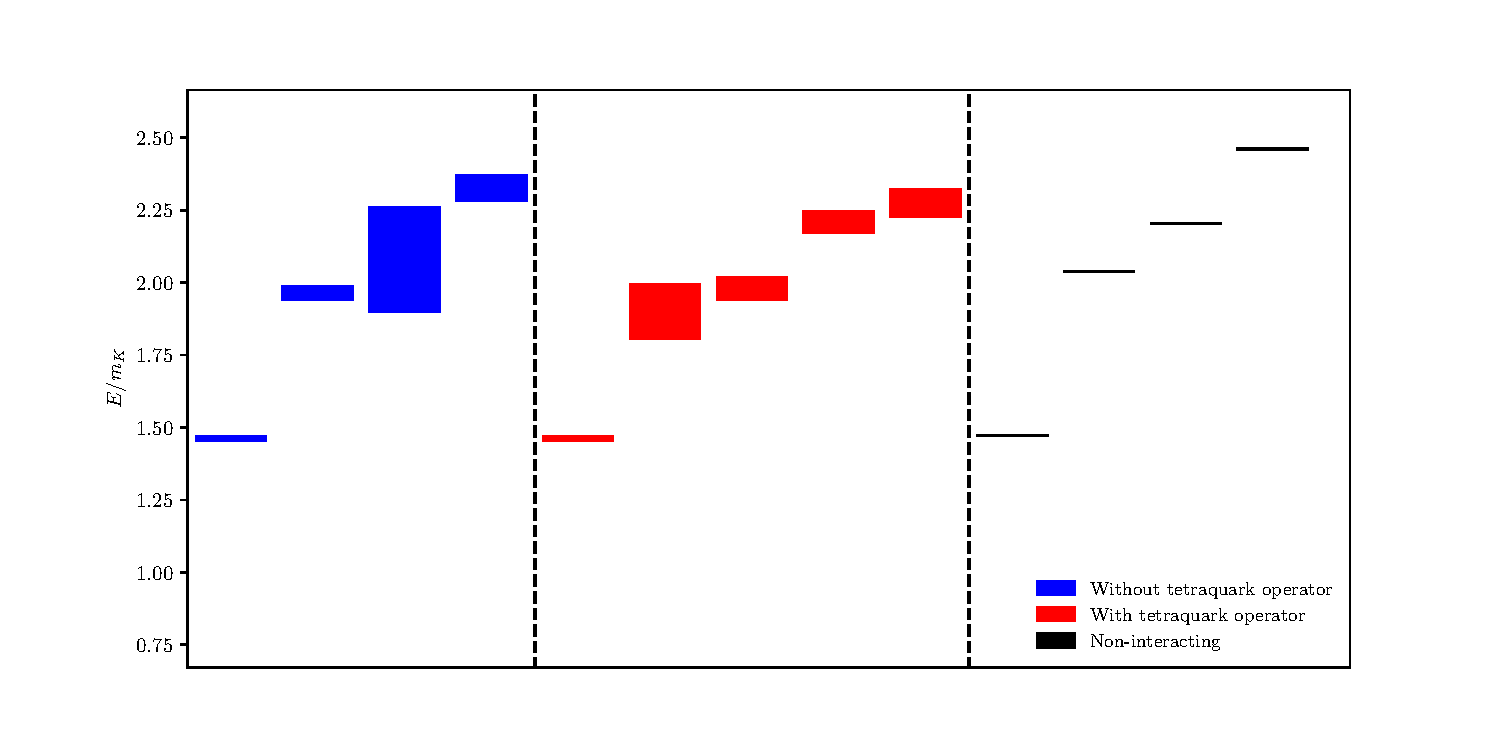
\includegraphics[scale=0.6]{figures/a1g_staircase.pdf}
  \caption{The first five and six levels of the spectrum in the $\kappa$ at-rest symmetry channel. On the left: the spectrum obtained using a basis with no tetraquark operators. In the middle: the spectrum obtained using one tetraquark operator. On the right: non-interacting levels shown for reference, where $(0)$ denotes to particles at rest, and $(1)$ denotes particles with unit momentum, and $(2)$ denotes particles with two units of squared momentum.}\label{fig:kappa_spectrum}
\end{figure}
\begin{figure}
  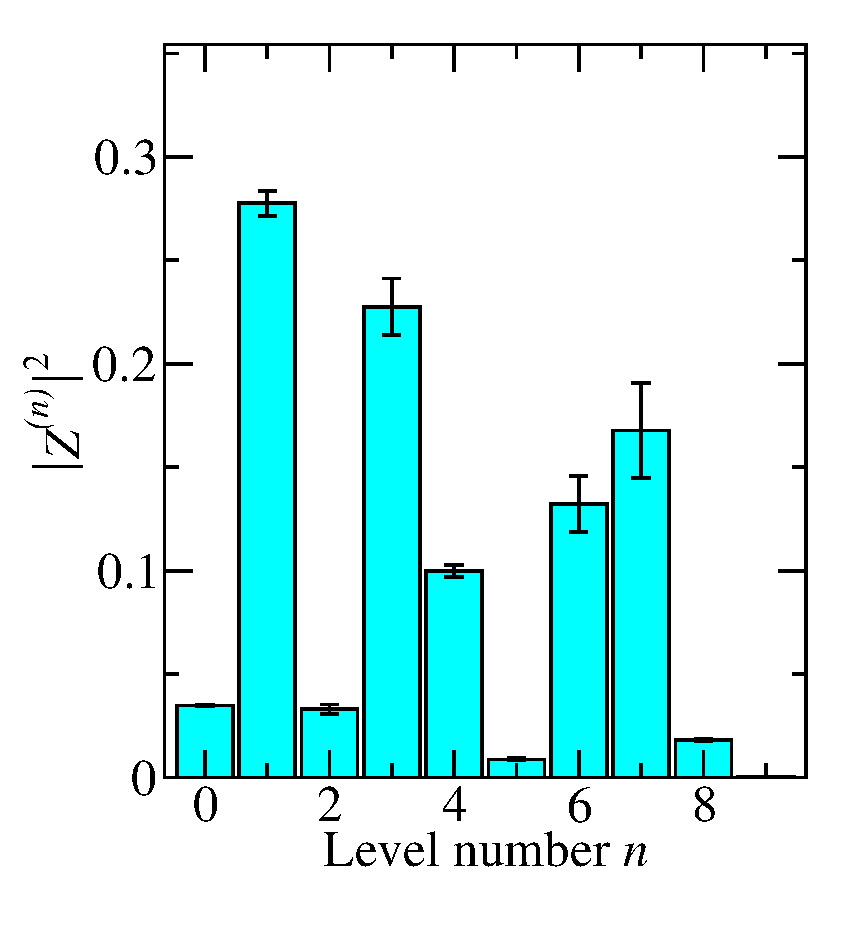
\includegraphics[scale=0.5]{figures/zfactors_a1g/zfactor_tqsuss2m-P000-A1g_1-SS_7.pdf}
  \caption{The overlap factors for the tetraquark operator used to produce the extra level in the $\kappa$ symmetry channel.}\label{fig:zkappa}
\end{figure}
\subsection{$a_0(980)$ Channel}
We summarize results obtained by fitting a spectrum in the $a_0(980)$ at-rest symmetry channel for again for two operator bases as in the $\kappa$ channel. Figure \ref{fig:a0_spectrum} shows the spectrum with and without the inclusion of a tetraquark operator in the basis. The tetraquark operator is of the flavor structure \textit{antilight-light-antilight-light}, and was also of the antisymmetric form in (\ref{eq:tsta}). We again see an extra level appear when we include a tetraquark operator. Again, overlap factors are shown for the tetraquark operator, and significant overlaps with the additional level can be seen in Figure~\ref{fig:za0}. This again suggests there is a state in our lattice spectrum that shares quantum numbers with the $a_0(980)$ resonance, and that has tetraquark content. As in the $\kappa$-channel case, evidence for or against the $a_0(980)$ having tetraquark content will have to wait for future scattering studies done using this data.
\begin{figure}
  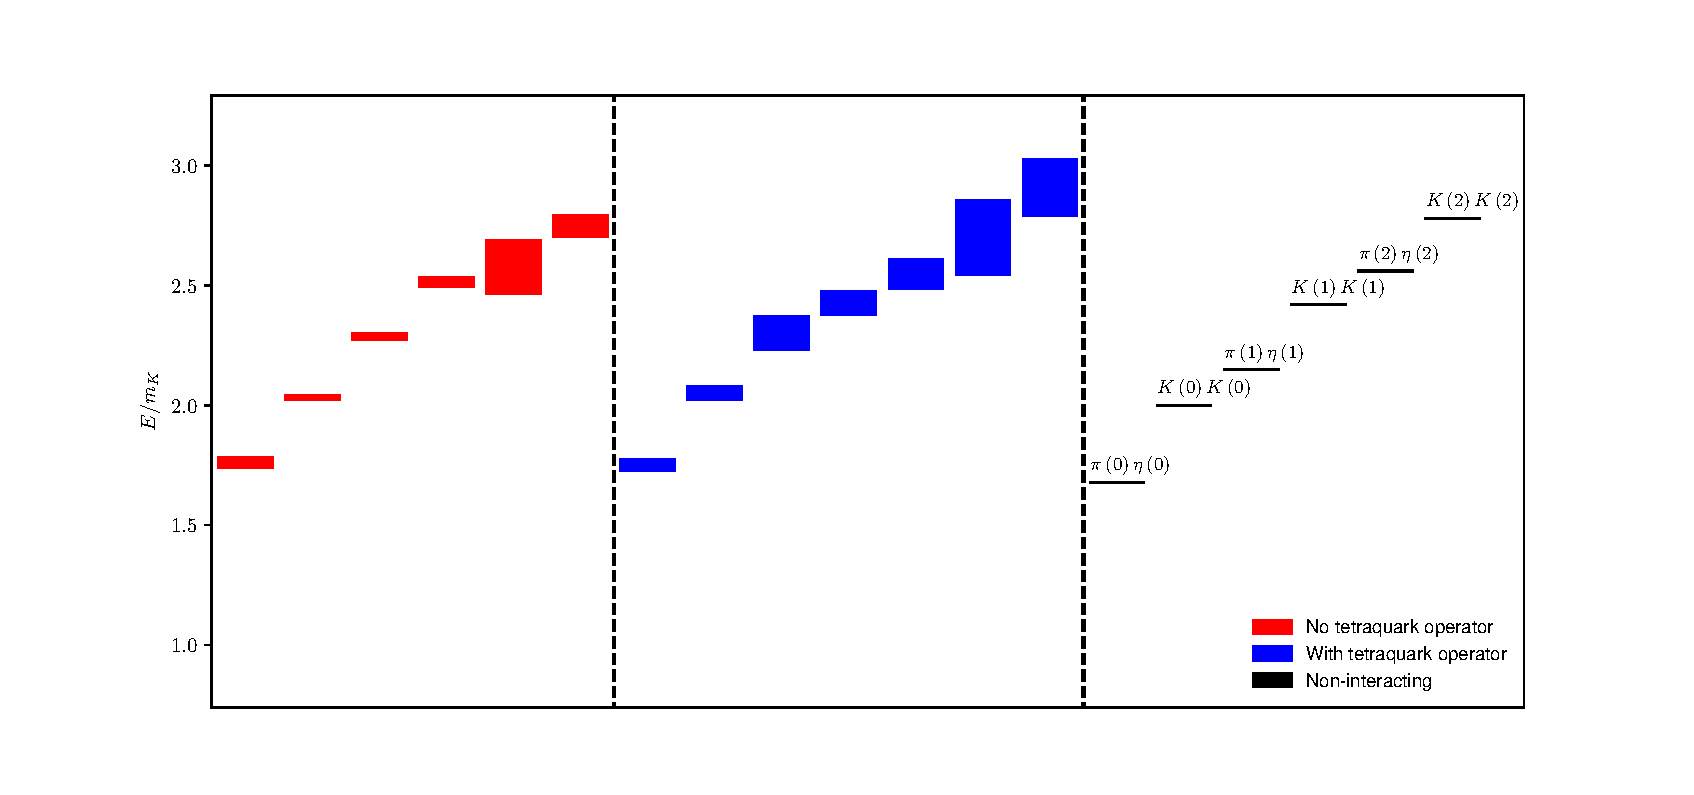
\includegraphics[scale=0.6]{figures/a1gm_staircase.pdf}
  \caption{The first six and seven levels of the spectrum in the $a_0(980)$ at-rest symmetry channel. On the left: the spectrum obtained using a basis with no tetraquark operators. In the middle: the spectrum obtained using one tetraquark operator. On the right: non-interacting levels shown for reference, where $(0)$ denotes to particles at rest, and $(1)$ denotes particles with unit momentum, and $(2)$ denotes particles with two units of squared momentum.}\label{fig:a0_spectrum}
\end{figure}
\begin{figure}
  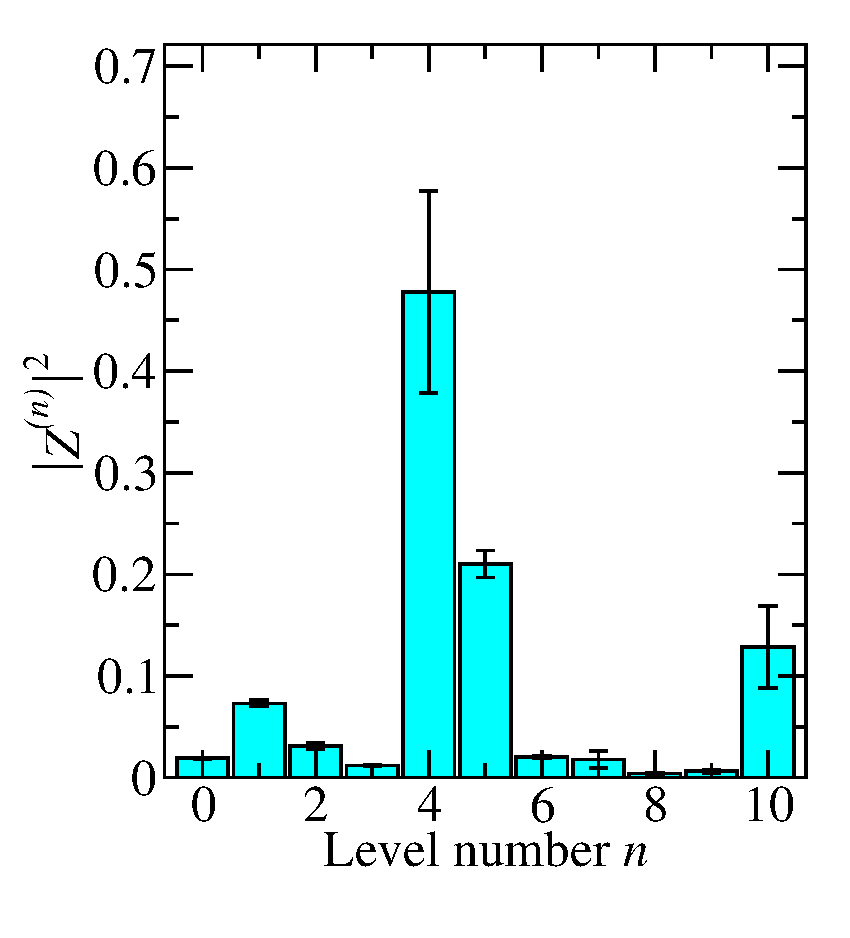
\includegraphics[scale=0.5]{figures/zfactors_a1gm/zfactor_uudu3m_SS_3.pdf}
  \caption{The overlap factors for the tetraquark operator used to produce the extra level in the $a_0(980)$ symmetry channel.}\label{fig:za0}
\end{figure}